\section{Opdrachtbeschrijving}
In het kader van ons bachelorproject ontwikkelen we een wagentje dat autonoom zo snel mogelijk een raceparcours kan afleggen. Dit parcours bestaat uit een zwarte ondergrond afgebakend door volle witte lijnen en een witte stippellijn in het midden, een voorbeeld hiervan ziet u in figuur~\vref{fig:parcoursvoorbeeld}. Ons wagentje mag niet buiten de volle witte lijnen van het parcours treden. Tevens zullen er op het traject verschillende RFID-tags geplaatst worden die door het voertuig ingelezen moeten worden. Eveneens moet er een manier voorzien worden om de snelheid van het voertuig te meten. De ingelezen tags en opgemeten snelheid moet ten slotte nog verzonden worden naar een Raspberry Pi. Voor het aanschaffen van nodige hardware krijgen we 50 euro ter beschikking.\\
\begin{figure}[H]
	\centering
	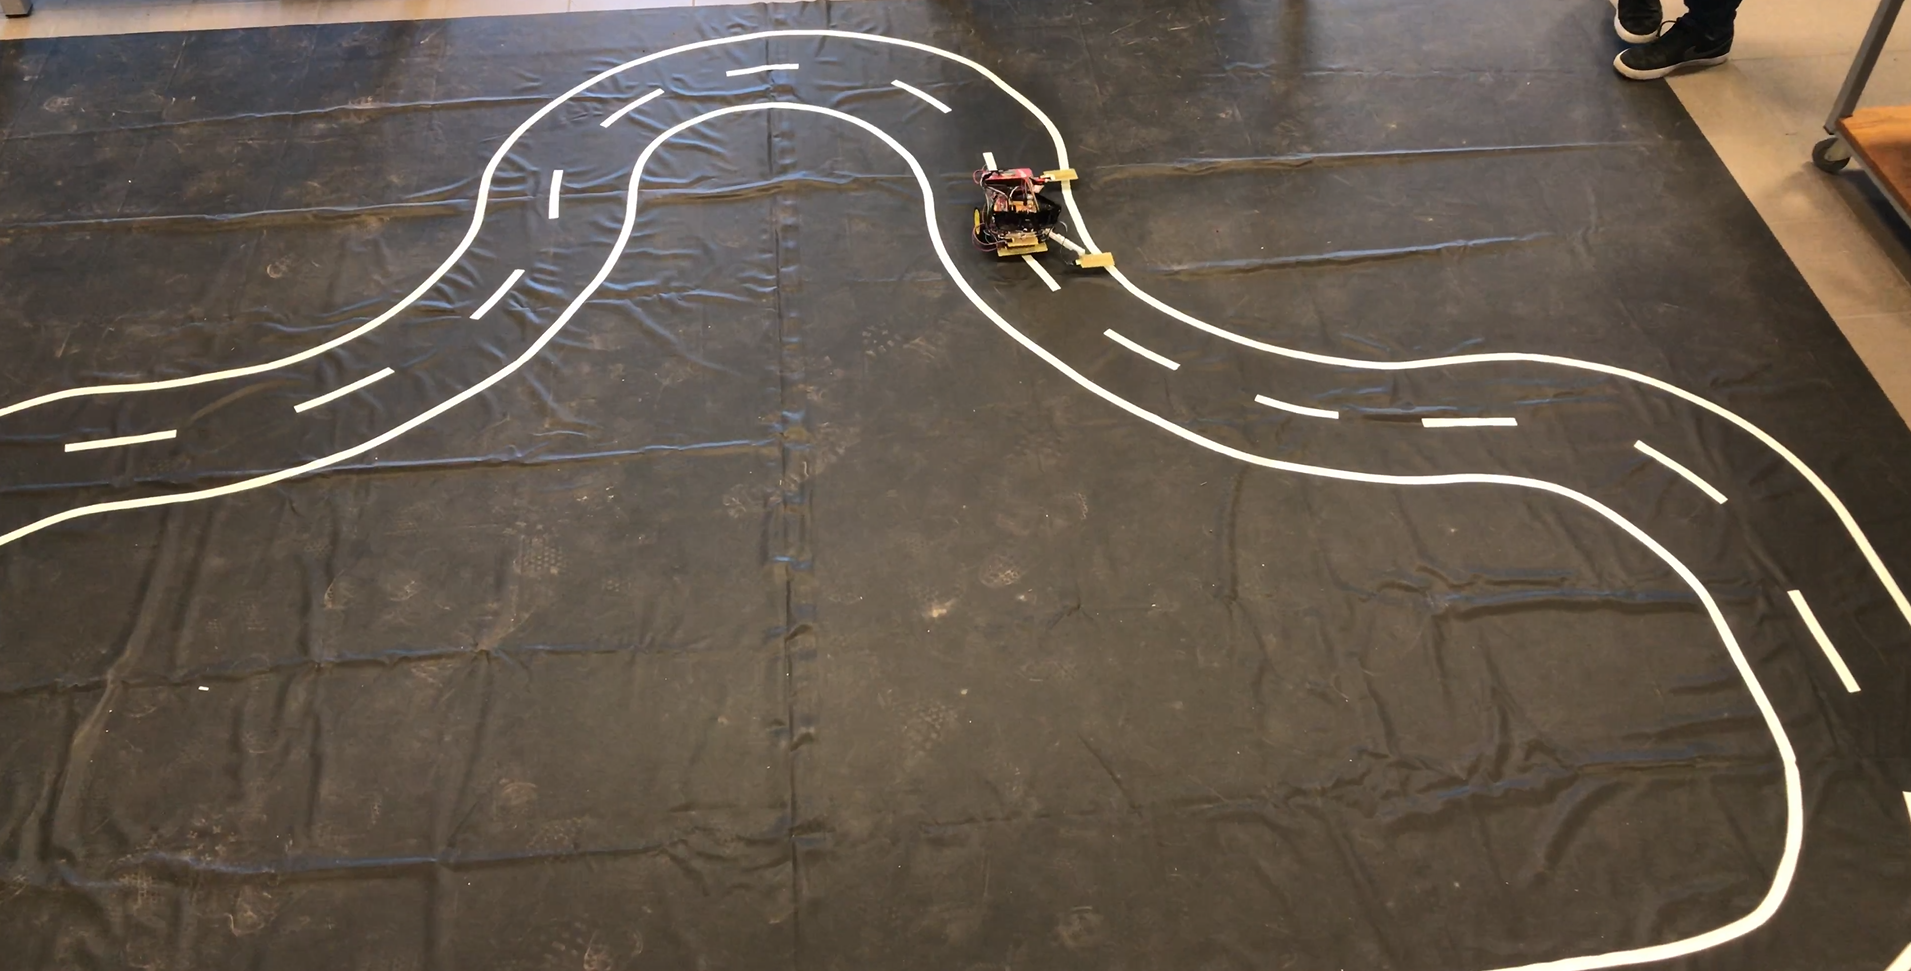
\includegraphics[width=\textwidth]{parcoursvoorbeeld.png}
	\caption{Voorbeeld parcours dat ons wagentje dient af te leggen}
	\label{fig:parcoursvoorbeeld}
\end{figure}
\subsection{Hardware}
We krijgen reeds een wagentje met twee motoren en een batterij om te beginnen.
Voor het prototypen en testen mogen we gebruik maken van een Arduino Uno met motor shield, eenn belangrijk deel van de opdracht bestaat er uit deze Arduino \'en motor shield te vervangen door \'e\'en custom board.
Qua hardware moeten we dus nog de custom board ontwikkelen, sensoren voorzien en uiteraard ook modules aanschaffen voor (Bluetooth) communicatie met de RPi en het inlezen van RFID-tags.\\
\subsection{Software}
De besproken hardware moet natuurlijk ook correct aangestuurd worden door software. Dit zal gebeuren aan de hand van Arduino-code ondersteund door C/C++ libraries. In deze software moeten voorzieningen getroffen worden voor het aansturen van de motoren, het inlezen van sensoren, communicatie met Raspberry Pi,...
Aan de kant van de Raspberry Pi zullen we verbinding moeten maken met ons wagentje en de data die doorgestuurd wordt afprinten op het scherm.


\section{Doelstellingen}
De belangrijkste doelstellingen van ons project zijn dus de volgende:
\begin{itemize}
	\item Voertuig autonoom laten het parcours afleggen
	\item Custom board ontwerpen om Arduino en motorshield te vervangen
	\item Snelheid van het wagentje meten
	\item RFID-lezer voorzien voor het uitlezen van tags op het parcours
	\item Communicatie (Bluetooth) tussen Arduino en Raspberry Pi 3 realiseren
\end{itemize}
\section{Structuur}
We beginnen dit verslag met een bespreking van onze planning, taakverdeling en gemaakte onkosten. Daarna behandelen we de gebruikte hardware en software om deze aan te sturen in meer detail. Vervolgens overleggen we de problemen en moeilijkheden die we doorheen het project ondervonden. Hierna volgt nog een evalutie van onze coach, Bert Cox. Ten slotte sluiten we af met een besluit omtrent het project waarin we bespreken wat we hebben bijgeleerd, wat er beter kan/kon,...